\documentclass[12pt]{article}
%\usepackage[utf8]{inputenc}
%\documentclass[UTF8]{ctexart}
%\usepackage[UTF8, heading = false, scheme = plain]{ctex}
\usepackage{geometry}
%geometry{a4paper,scale=0.9}
\geometry{a4paper,left=1cm,right=1cm,top=1cm,bottom=2cm}
\usepackage{amsfonts}
\usepackage{color}
\usepackage{url}
%\usepackage{biblatex}
\usepackage{amsmath}
\usepackage{amssymb}
\usepackage{latexsym}
\usepackage[linesnumbered,ruled,lined]{algorithm2e}
\usepackage{cite}
%\addbibresource{ref.bib}
%\bibliography{ref.bib}
\usepackage{caption}
\usepackage{graphicx, subfig}
\usepackage{float}
%\usepackage[fontset=ubuntu]{ctex}
%\usepackage{fontspec}
\usepackage{xeCJK}
%\usepackage[colorlinks,
%anchorcolor=black,
%citecolor=black]{hyperref}
%\setmainfont{SimSun}
\usepackage[section]{placeins}
\usepackage{enumitem}
\usepackage{framed}
\usepackage[framemethod=TikZ]{mdframed}
\usepackage{indentfirst}
\usepackage{setspace}%使用间距宏包
\linespread{1.5}

\title{Embedding 讨论}
\author{leolinuxer}
%\date{June 2020}

\begin{document}
%\setlength{\parindent}{0pt}
\maketitle
\tableofcontents

\section{Embedding简介\cite{Embedding_From_Word2Vec_To_Item2Vec}}
\subsection{什么是embedding}
简单来说,embedding就是用一个低维的向量表示一个物体,可以是一个词,或是一个商品,或是一个电影等等。这个embedding向量的性质是能使距离相近的向量对应的物体有相近的含义,比如 Embedding(复仇者联盟)和Embedding(钢铁侠)之间的距离就会很接近,但 Embedding(复仇者联盟)和Embedding(乱世佳人)的距离就会远一些。

除此之外Embedding甚至还具有数学运算的关系,比如Embedding(马德里)-Embedding(西班牙)+Embedding(法国)≈Embedding(巴黎)

言归正传,Embedding能够用低维向量对物体进行编码还能保留其含义的特点非常适合深度学习。在传统机器学习模型构建过程中,我们经常使用one hot encoding对离散特征,特别是id类特征进行编码,但由于one hot encoding的维度等于物体的总数,比如阿里的商品one hot encoding的维度就至少是千万量级的。这样的编码方式对于商品来说是极端稀疏的,甚至用multi hot encoding对用户浏览历史的编码也会是一个非常稀疏的向量。而深度学习的特点以及工程方面的原因使其不利于稀疏特征向量的处理。因此如果能把物体编码为一个低维稠密向量再喂给DNN,自然是一个高效的基本操作。

\subsection{使 embedding 空前流行的 word2vec}
对word的vector表达的研究早已有之,但让embedding方法空前流行,我们还是要归功于google的word2vec。我们简单讲一下word2vec的原理,这对我们之后理解AirBnB对loss function的改进至关重要。

既然我们要训练一个对 word 的语义表达,那么训练样本显然是一个句子的集合。假设其中一个长度为 $T$ 的句子为$w_1, w_2, \cdots, w_T$ 。这时我们假定每个词都跟其相邻的词的关系最密切,换句话说每个词都是由相邻的词决定的(CBOW模型的动机),或者每个词都决定了相邻的词(Skip-gram模型的动机)。如下图,CBOW的输入是 $w_t$ 周边的词,预测的输出是$w_t$,而Skip-gram则反之,经验上讲Skip-gram的效果好一点,所以本文从Skip-gram模型出发讲解模型细节。

\begin{figure}[H]
    \centering
    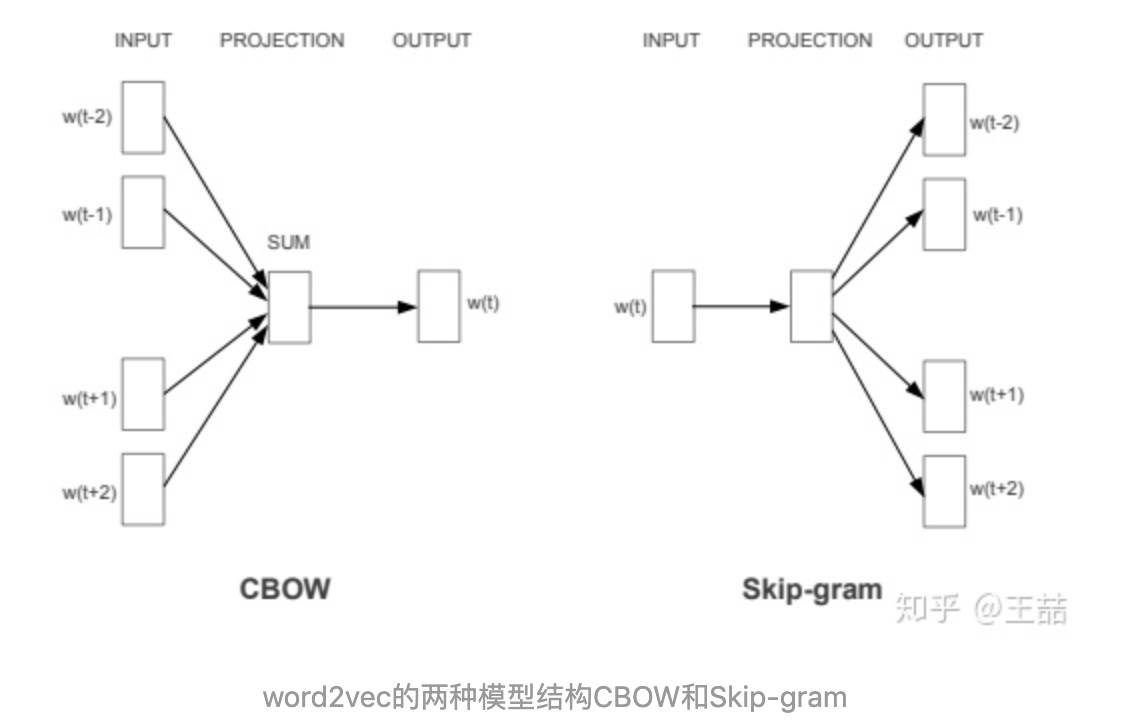
\includegraphics[width=.8\textwidth]{fig/Embedding_Word2vec_Skip-gram_CBOW.png}
\end{figure}

那么为了产生模型的正样本,我们选一个长度为$2c+1$(目标词前后各选$c$个词)的滑动窗口,从句子左边滑倒右边,每滑一次,窗口中的词就形成了我们的一个正样本。

有了训练样本之后我们就可以着手定义优化目标了,既然每个词$w_t$都决定了相邻词 $w_{t+j}$,基于极大似然,我们希望所有样本的条件概率 $p(w_{t+j}|w_t)$ 之积最大,这里我们使用log probability。我们的目标函数有了:
$$
\frac{1}{T} \sum_{t=1}^T\sum_{-c \le j \le c, j \neq 0} \log{p(w_{t+j}|w_t)}
$$

接下来的问题是怎么定义 $p(w_{t+j}|w_t)$ ,作为一个多分类问题,最简单最直接的方法当然是直接用softmax函数,我们又希望用向量$w_t$ 表示每个词 w,用词之间的距离 $v_i^Tv_i$ 表示语义的接近程度,那么我们的条件概率的定义就可以很直观的写出。
$$
P(w_O|w_I) = \frac{\text{exp}({v'}_{w_O}^Tv_{w_I})}{\sum_{w=1}^W\text{exp}({{v'}_{w_O}^Tv_{w_I}})}
$$

看到上面的条件概率公式,很多同学可能会习惯性的忽略一个事实,就是

\textbf{我们用 $w_t$ 去预测 $w_{t+j}$ ,但其实这二者的向量表达并不在一个向量空间内。}

就像上面的条件概率公式写的一样,$v'_w$ 和 $v_w$ 分别是词w的输出向量表达和输入向量表达。那什么是输入向量表达和输出向量表达呢?我们画一个word2vec的神经网络架构图就明白了。
\begin{figure}[H]
    \centering
    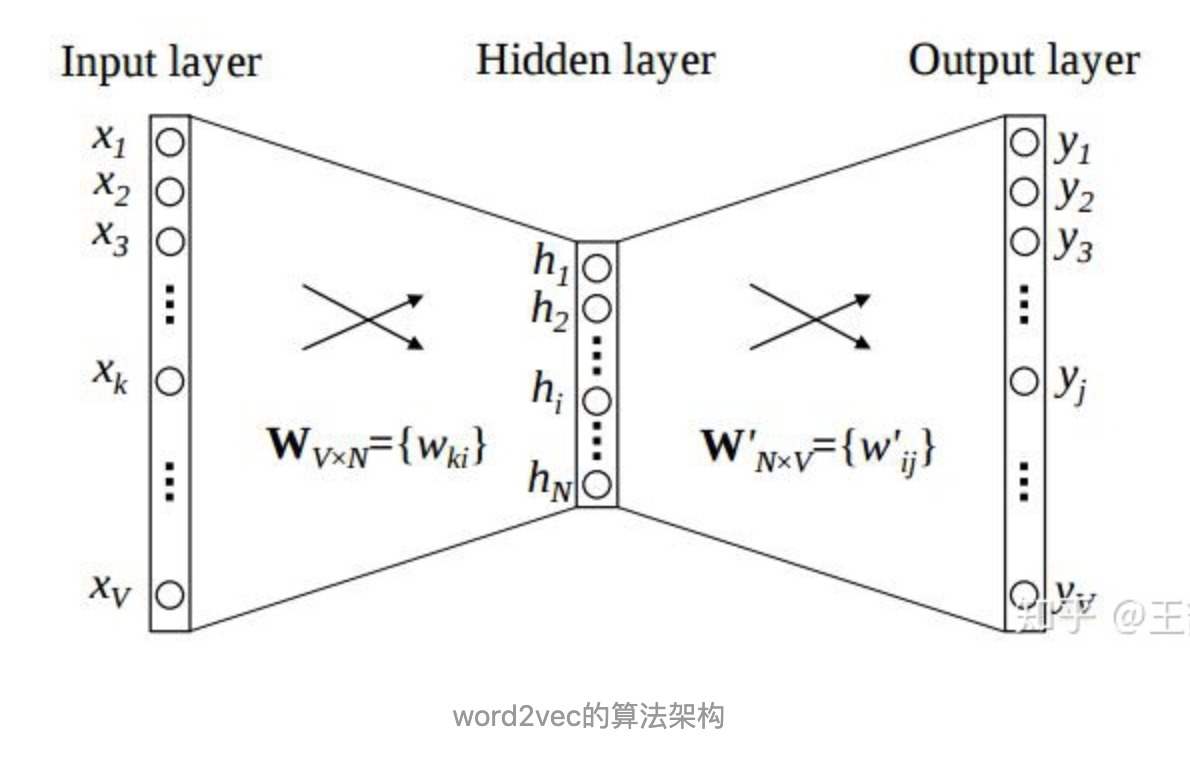
\includegraphics[width=.8\textwidth]{fig/Word2Vec_Algorithm_Structure.png}
\end{figure}

根据 $p(w_{t+j}|w_t)$ 的定义,我们可以把两个vector的乘积再套上一个softmax的形式转换成上面的神经网络架构(需要非常注意的一点是hidden layer的激活函数,大家要思考一下,到底是sigmoid函数还是普通的线性函数,为什么?)。在训练过程中我们就可以通过梯度下降的方式求解模型参数了。那么上文所说的输入向量表达就是input layer到hidden layer的权重矩阵$W_{V\times N}$ ,而输出向量表达就是hidden layer到output layer的权重矩阵$W'_{N\times V}$ 。

\textbf{那么到底什么是我们通常意义上所说的词向量 $v_w$ 呢?}

其实就是我们上面所说的输入向量矩阵 $W_{V\times N}$ 中每一行对应的权重向量。于是这个权重矩阵自然转换成了word2vec的lookup table。
\begin{figure}[H]
    \centering
    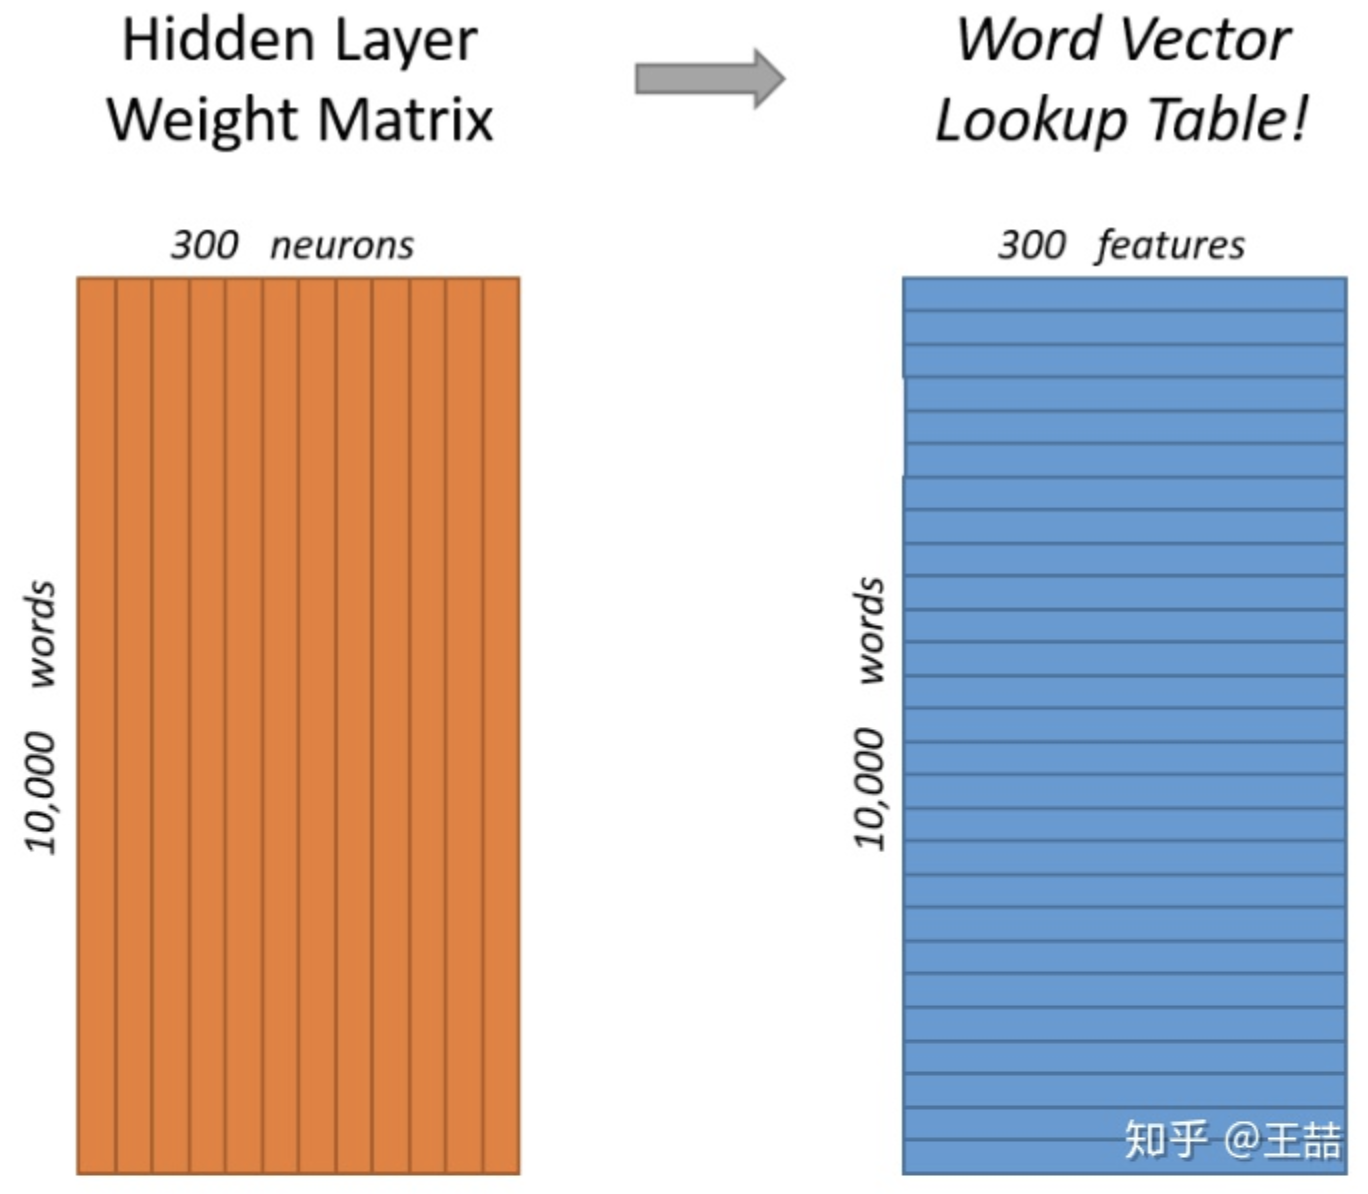
\includegraphics[width=.6\textwidth]{fig/Word2Vec_Lookup_Table.png}
\end{figure}

当然在训练word2vec的过程中还有很多工程技巧,比如用negative sampling或Hierarchical Softmax减少词汇空间过大带来的计算量,对高频词汇进行降采样避免对于这些低信息词汇的无谓计算等。在具体实现的时候最好参考Google的原文 Distributed Representations of Words and Phrases and their Compositionality

\subsection{从word2vec到item2vec}
在word2vec诞生之后,embedding的思想迅速从NLP领域扩散到几乎所有机器学习的领域,我们既然可以对一个序列中的词进行embedding,那自然可以对用户购买序列中的一个商品,用户观看序列中的一个电影进行embedding。而广告、推荐、搜索等领域用户数据的稀疏性几乎必然要求在构建DNN之前对user和item进行embedding后才能进行有效的训练。

具体来讲,如果item存在于一个序列中,item2vec的方法与word2vec没有任何区别。而如果我们摒弃序列中item的空间关系,在原来的目标函数基础上,自然是不存在时间窗口的概念了,取而代之的是item set中两两之间的条件概率:
$$
\frac{1}{K}\sum_{i=1}^K\sum_{j \neq i}^K \log{p(w_j|w_i)}
$$

具体可以参考item2vec的原文 Item2Vec:Neural Item Embedding for Collaborative Filtering

但embedding的应用又远不止于此,事实上,由于我们也可以把输出矩阵的列向量当作item embedding,这大大解放了我们可以用复杂网络生成embedding的能力。读过我专栏上一篇文章 YouTube深度学习推荐系统的十大工程问题 的同学肯定知道,YouTube在serve其candidate generation model的时候,只将最后softmax层的输出矩阵的列向量当作item embedding vector,而将softmax之前一层的值当作user embedding vector。在线上serving时不用部署整个模型,而是只存储user vector和item vector,再用最近邻索引进行快速搜索,这无疑是非常实用的embedding工程经验,也证明了我们可以用复杂网络生成user和item的embedding。

\begin{figure}[H]
    \centering
    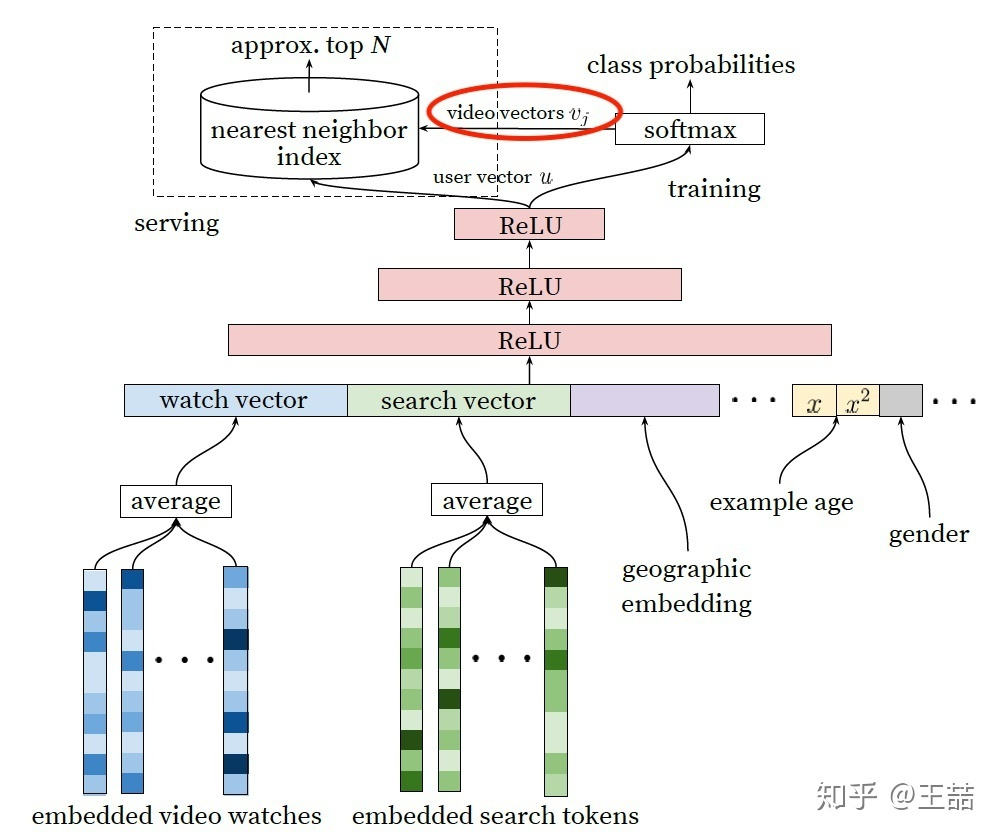
\includegraphics[width=.8\textwidth]{fig/Embedding_In_Youtube_2.jpg}
\end{figure}

KDD 2018 best paper Real-time Personalization using Embeddings for Search Ranking at Airbnb 也介绍了Airbnb的embedding最佳实践。

\section{Embedding在深度推荐系统中的3大应用方向
\cite{Three_Application_Of_Embedding_In_Reference_System}}

在深度学习推荐系统中,Embedding有三个主要的应用方向:
\begin{itemize}
\setlength{\itemsep}{0pt}
\setlength{\parsep}{0pt}
\setlength{\parskip}{0pt}
    \item 在深度学习网络中作为Embedding层,完成从高维稀疏特征向量到低维稠密特征向量的转换;
    \item 作为预训练的Embedding特征向量,与其他特征向量连接后一同输入深度学习网络进行训练;
    \item 通过计算用户和物品的Embedding相似度,Embedding可以直接作为推荐系统或计算广告系统的召回层或者召回方法之一;
\end{itemize}

\subsection{深度学习网络中的Embedding层}
由于高维稀疏特征向量天然不适合多层复杂神经网络的训练,因此如果使用深度学习模型处理高维稀疏特征向量,几乎都会在输入层到全连接层之间加入Embedding层完成高维稀疏特征向量到低维稠密特征向量的转换。典型的例子是微软的Deep Crossing模型和Google的Wide\&Deep模型的深度部分。
\begin{figure}[H]
    \centering
    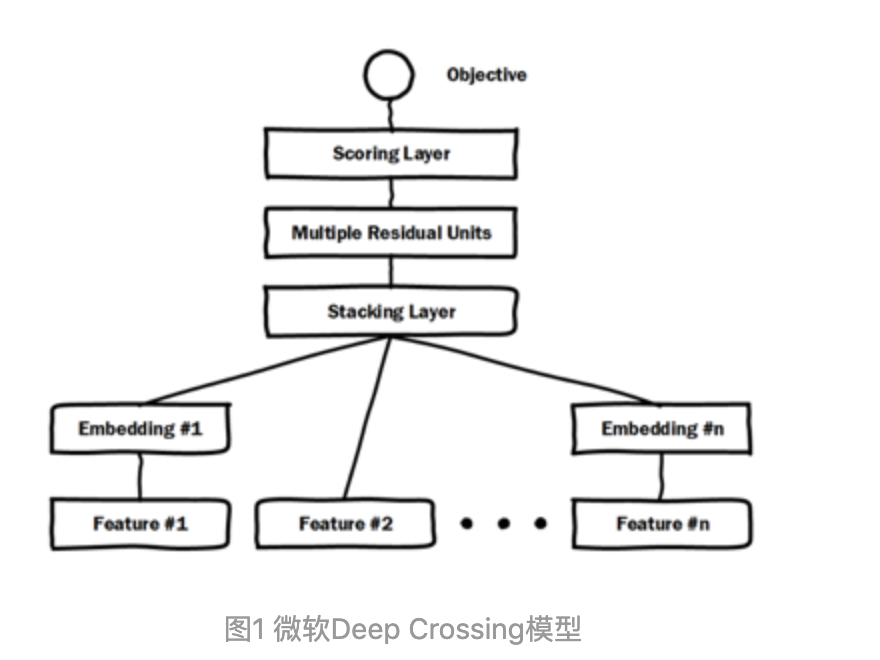
\includegraphics[width=.8\textwidth]{fig/Microsoft_Deep_Crossing_Strucure.png}
\end{figure}
\begin{figure}[H]
    \centering
    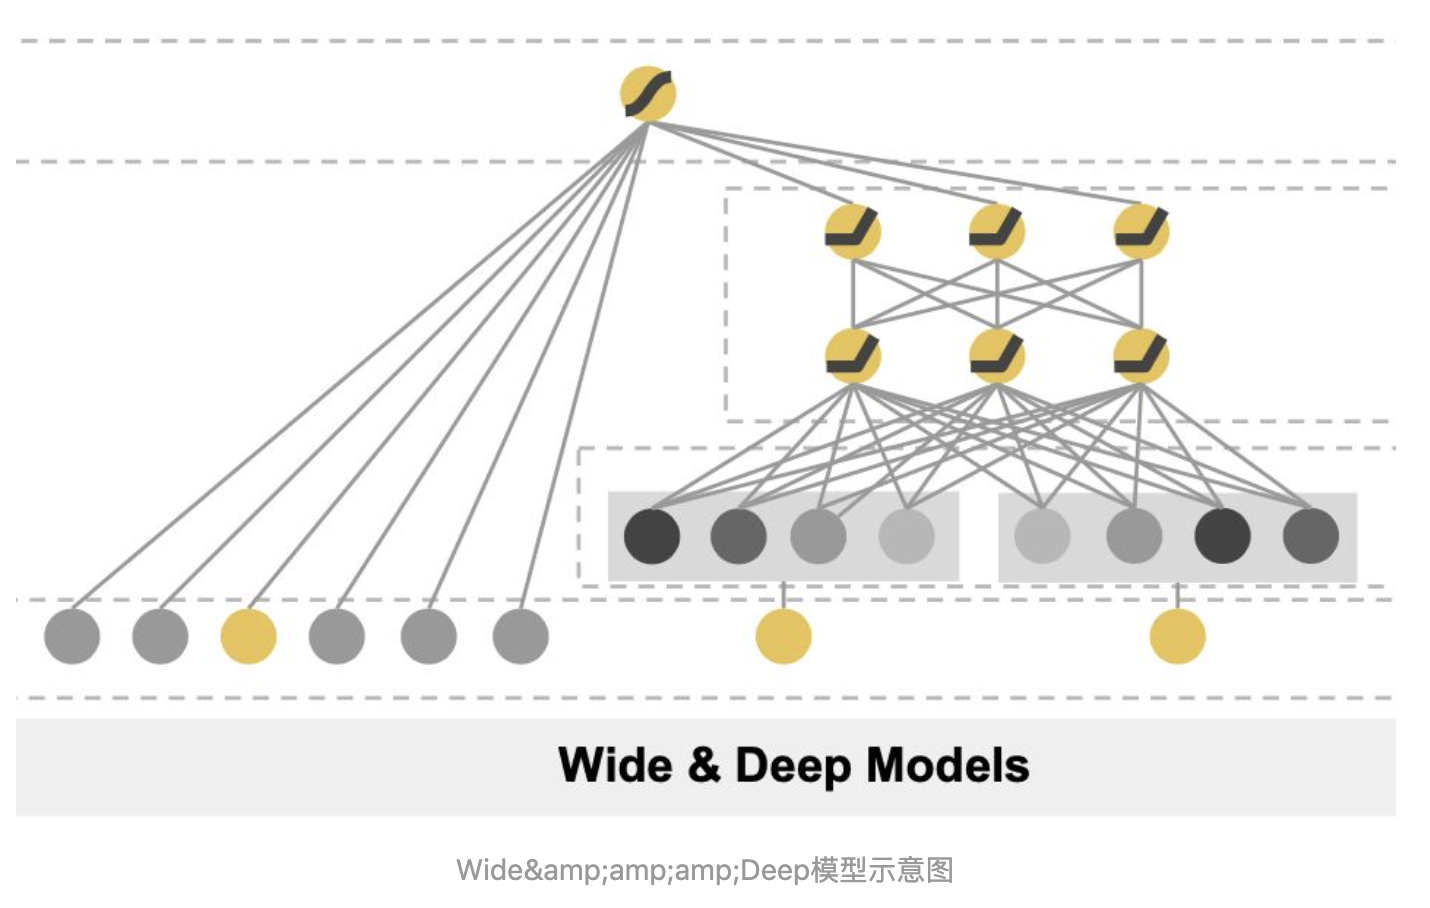
\includegraphics[width=.8\textwidth]{fig/Wide_Deep_Structure.png}
\end{figure}

图1中可以清晰的看到Deep Crossing模型中的Embedding层将每一个Feature转换成稠密向量,图2Wide\&Deep模型中Deep部分的Dense Embeddings层同样将稀疏特征向量进行转换。广义来说,Embedding层的结构可以比较复杂,只要完成高维向量的降维就可以了,但一般为了节省训练时间,深度神经网络中的Embedding层是一个高维向量向低维向量的直接映射(如图3)。
\begin{figure}[H]
    \centering
    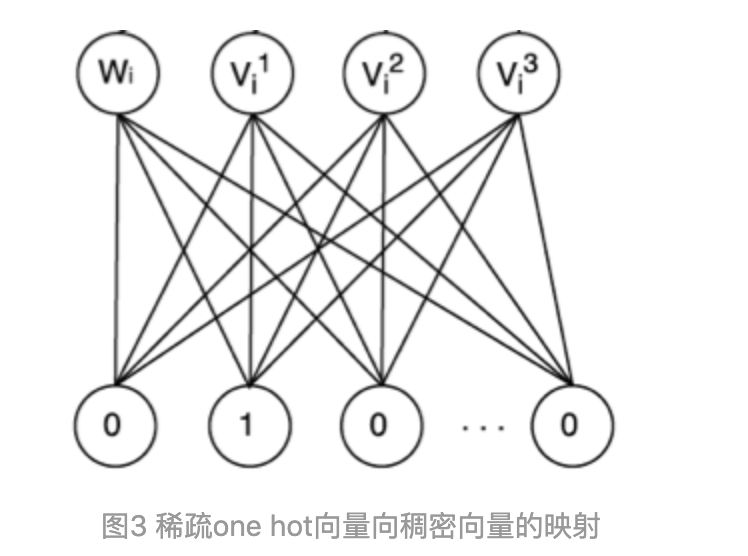
\includegraphics[width=.5\textwidth]{fig/Embedding_From_One_Hot_Example.png}
\end{figure}

一般来说,推荐系统的输入向量中包含大量稀疏的 one hot 特征,图3展示了典型的稀疏向量向稠密embedding向量的最简单的embedding层结构。

用矩阵的形式表达Embedding层,本质上是求解一个 m(输入高维稀疏向量的维度) x n(输出稠密向量的维度)维的权重矩阵的过程。如果输入向量是 one-hot 特征向量的话,权重矩阵中的列向量即为相应维度one-hot特征的embedding向量。

将Embedding层与整个深度学习网络整合后一同进行训练是理论上最优的选择,因为上层梯度可以直接反向传播到输入层,模型整体是自洽和统一的。但这样做的缺点同样显而易见的,由于Embedding层输入向量的维度甚大,Embedding层的加入会拖慢整个神经网络的收敛速度。

\begin{framed}
这里可以做一个简单的计算。假设输入层维度是100,000,embedding输出维度是32,上层再加5层32维的全连接层,最后输出层维度是10,那么输出层到embedding层的参数数量是32*100,000= 3,200,000,其余所有层的参数总数是 (32*32)*4+32*10=4416。那么embedding层的权重总数占比是 3,200,000 / (3,200,000 + 4416) = 99.86\%。
\end{framed}

也就是说embedding层的权重占据了整个网络权重的绝大部分。那么训练过程可想而知,大部分的训练时间和计算开销都被Embedding层所占据。正因为这个原因,Embedding层往往采用预训练的方式完成。

\subsection{Embedding的预训练方法}
通过上面对Embedding层的介绍,同学们肯定已经知道Embedding层的训练开销是巨大的。为了解决这个问题,Embedding的训练往往独立于深度学习网络进行。在得到稀疏特征的稠密表达之后,再与其他特征一起输入神经网络进行训练。典型的采用Embedding预训练方法的模型是FNN(如图4)。
\begin{figure}[H]
    \centering
    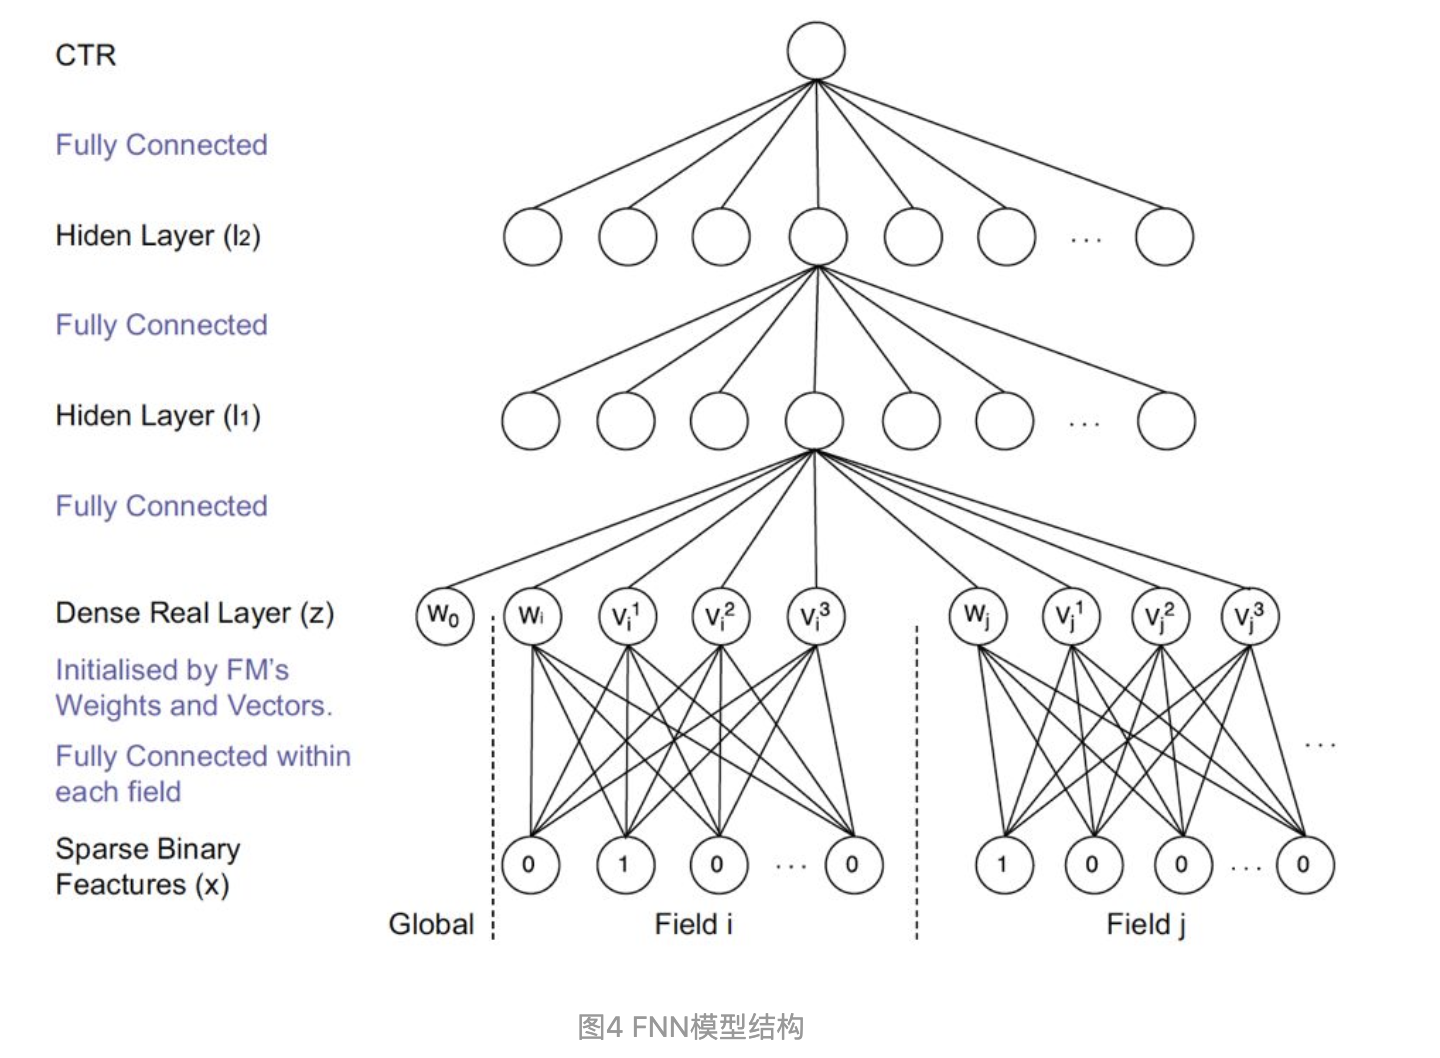
\includegraphics[width=.8\textwidth]{fig/FNN_Structure.png}
\end{figure}

FNN利用了FM训练得到的物品向量,作为Embedding层的初始化权重,从而加快了整个网络的收敛速度。在实际工程中,直接采用FM的物品向量作为Embedding特征向量输入到后续深度学习网络也是可行的办法。

再延伸一点讲,Embedding的本质是建立高维向量到低维向量的映射,而“映射”的方法并不局限于神经网络,实质上可以是任何异构模型,这也是Embedding预训练的另一大优势,就是可以采用任何传统降维方法,机器学习模型,深度学习网络完成embedding的生成。

典型的例子是2013年Facebook提出的著名的GBDT+LR的模型,其中GBDT的部分本质上也是完成了一次特征转换,可以看作是利用GBDT模型完成Embedding预训练之后,将Embedding输入单层神经网络进行CTR预估的过程。

\begin{figure}[H]
    \centering
    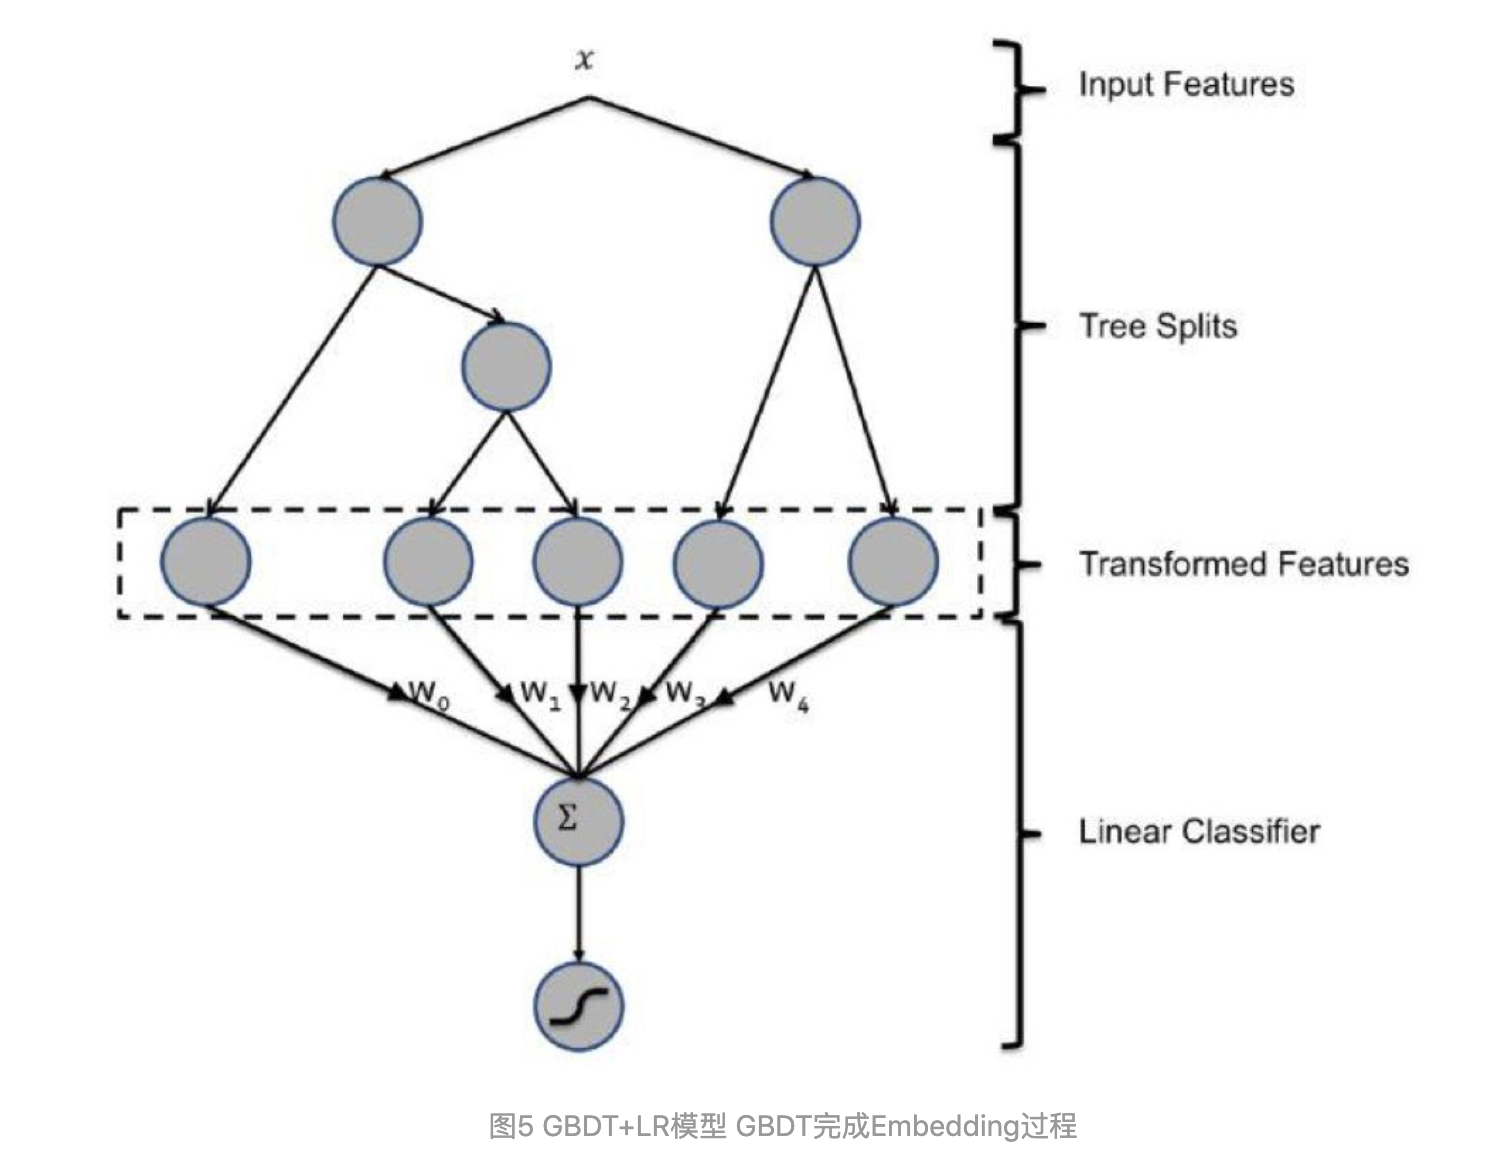
\includegraphics[width=1\textwidth]{fig/Embedding_GBDT_LR.png}
\end{figure}

2015年以来,随着大量Graph Embedding技术的发展,Embedding本身的表达能力进一步增强,而且能够将各类特征全部融合进Embedding之中,这使Embedding本身成为非常有价值的特征。这些特点都使Embedding预训练成为更被青睐的技术途径。

诚然,将Embedding过程与深度网络的训练过程割裂,必然会损失一定的信息,但训练过程的独立也带来了训练灵活性的提升。举例来说,由于物品或用户的Embedding天然是比较稳定的(因为用户的兴趣、物品的属性不可能在几天内发生巨大的变化),Embedding的训练频率其实不需要很高,甚至可以降低到周的级别,但上层神经网络为了尽快抓住最新的正样本信息,往往需要高频训练甚至实时训练。使用不同的训练频率更新Embedding模型和神经网络模型,是训练开销和模型效果二者之间权衡后的最优方案。

\subsection{embedding作为推荐系统或计算广告系统的召回层}
随着Embedding技术的进步,Embedding自身的表达能力也逐步增强,利用Embedding向量的相似性,直接将Embedding作为推荐系统召回层的方案越来越多的被采用。其中Youtube推荐系统召回层的解决方案是典型的做法。
\begin{figure}[H]
    \centering
    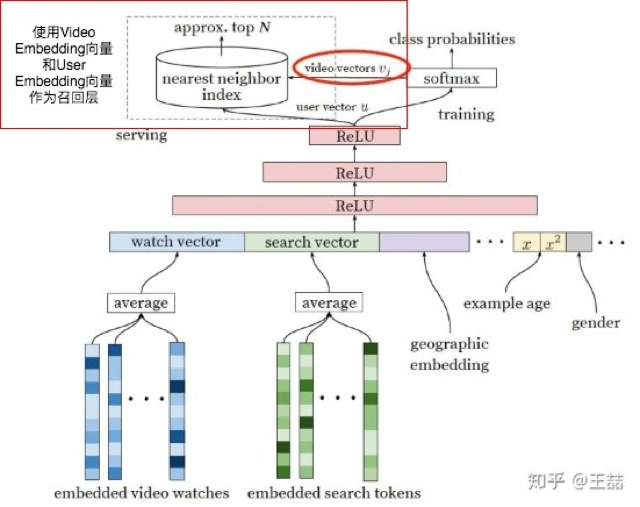
\includegraphics[width=1\textwidth]{fig/Embedding_In_Youtube.jpg}
\end{figure}

我曾经在文章《重读Youtube深度学习推荐系统论文,字字珠玑,惊为神文》中介绍过了Youtube利用深度学习网络生成Video Embedding和User Embedding的方法。利用最终的Softmax层的权重矩阵,每个Video对应的列向量就是其Item Embedding,而Softmax前一层的输出就是User Embedding。在模型部署过程中,没有必要部署整个深度学习网络来完成从原始特征向量到最终输出的预测过程,只需要将User Embedding和Item Embedding存储到线上内存数据库,通过内积运算再排序的方法就可以得到item的排名。这大大加快了召回层的召回效率。

\subsection{总结}
事实上,除了上述的三种主要的Embedding应用方向,业界对于Embedding的创新性研究不仅没有停止,而且有愈演愈烈之势,阿里的EGES,Pinterest的GNN应用,Airbnb基于Embedding的搜索模型等大量表达能力非常强的Embedding方法的诞生,使Embedding本身就已经成为了优秀的CTR模型和推荐系统模型。作为计算广告和推荐系统领域的从业者,无论如何强调Embedding的重要性都不过分。

\section{扩展阅读}
Embedding从入门到专家必读的十篇论文:\url{https://zhuanlan.zhihu.com/p/58805184}

%\printbibliography
\bibliography{../ref}
\bibliographystyle{IEEEtran}
\end{document}